\chapter{Speaker Models e Backend}
\label{ch:speakermodels}

\section{Applicazione del Deep Learning}
Nel contesto della ASR, come visto anche nel capitolo precedente, si è registrato un notevole interesse verso approcci basati su Deep Learning. 
Il Deep Learning (DL) grazie ad approcci e metodologie basate sul machine learning in generale, riusciamo a processare meglio le informazioni 
delle features estratte. \\
Il deep learning \cite{tirumala2016review} permette di poter elaborare le features ed estrarre rappresentazioni più complesse dei dati, permettendo quindi di realizzare dei
veri e propri \textbf{Speaker Models}. Gli speaker models costituiscono il nostro database, dove possiamo andare a salvare le caratteristiche o 
in generale le informazioni importanti per poter riconoscere gli utenti. Una considerazione importante va fatta sui modelli utilizzati, come le Deep Neural Network (DNN),
reti ricorrenti con memoria (come le Recurrent Neural Network, RNN, con Long Short Term Memory, LSTM) o reti che applicano filtri di convoluzione Convolutional Neural Network.
Sebbene le DNN siano quelle più semplici e di facile interpretazione, permettono semplicemente di estrarre pattern attraverso layer multistrato. Mentre, la combinazione
di reti RNN e CNN permette di unire i due principali vantaggi di queste reti: capacità di estrazione di features complesse applicando filtri convolutivi (tramite la CNN),
e capacità di memoria e ricordo (tramite la RNN con LSTM). In ogni caso, anche reti più complesse sono state proposte, sia per i task che per estrazione di embedding. 
Va infatti ricordato che queste reti fungono spesso anche da estrazione di embeddings, sulla base di features estratte precedentemente (ad esempio tramite MFCCs). \\
Un altro aspetto chaive, riguardando le immagini sugli schemi di funzionamento, è legato alla fase successiva di \textbf{pattern matching}. Questa parte spesso viene definita come
backend del sistema, dal momento che spesso questa fase avviene dopo che è stato effettuato l'\textbf{enrolment} del modello. Spesso come backend si preferisce lavorare con gli embeddings 
elaborati dalle reti di DL, che permettono di lavorare con informazioni più raffinate. Tipici backend prevedono l'applicazione di modelli come le Gaussian Mixture Models (GMM),
che usiamo per estrarre degli scores di similarità con cui valutare score di EER per stabilire l'affidabilità del modello stesso. \\
Gli autori di \cite{irum2019speaker} ad esempio hanno svolto un lavoro esaustivo sulla possibilità di applicare il Deep Learning nel task di Speaker Verification,
andando a riassumere quali sono i principali modelli utilizzati sia come speaker models che come backend. Una tabella riassuntiva difatti è portata in Fig.\ref{fig:studiopaper}.
Come si evince dallostudio condotto, spesso ci basiamo su score di similarità con distanza coseno o PLDA, avendo comunque sistemi basati su scores di un backend basato su
GMM-UBM (ovvero le \textbf{Gaussian Mixture Model - Universal Background Model}), che permette di realizzare un modello probabilistico che rappresenta la distribuzione di dati
come una combinazione di distribuzion gaussiane, andando quindi a modellare la voce (gli embeddings) di ogni speaker, difatti rappresentando un databse (Universal Background Model). 
\begin{figure}[ht]
    \centering
    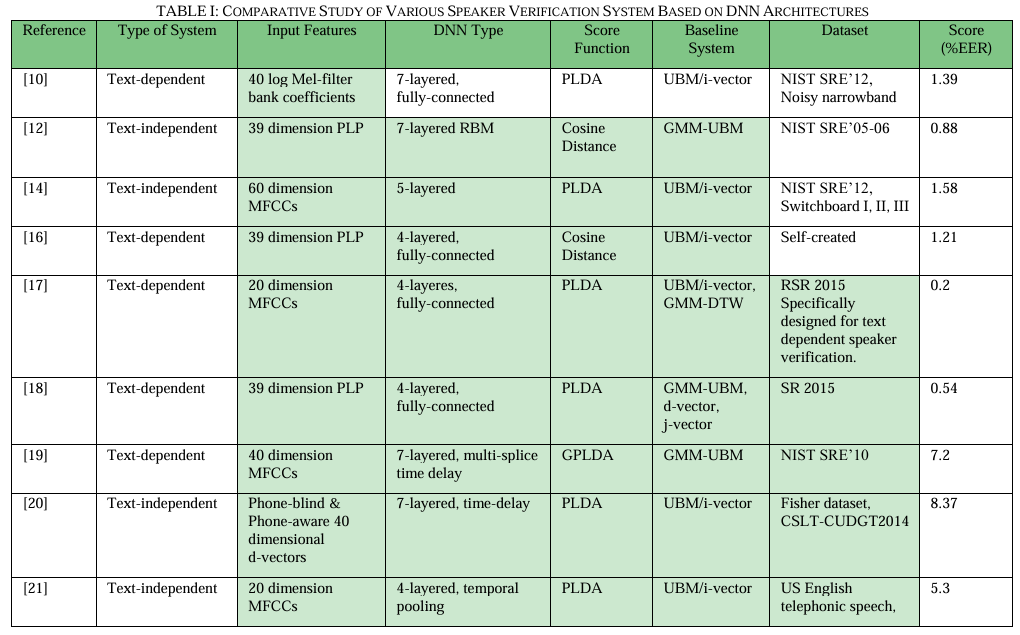
\includegraphics[width=1.0\textwidth]{./ch3/studio.png}
    \caption{Overview del Deep Learning applicato al problema, \cite{irum2019speaker}}
    \label{fig:studiopaper}
\end{figure}

\section{Metodologia del progetto}
Per la realizzazione del progetto abbiamo esplorato diverse strade basate sul deep learning, partendo comunque dal problema della speaker identification. 
Difatti, sulla base della speaker identification, possiamo poi usare la rete basata su deep learning stessa per poter identificare correttamente 
un utente tramite classificazione in termini di closed-set. Dopodiché siamo passati al task di speaker verification, partendo però dal modello addestrato che adesso funzionerà
da generatore di embeddings. Con questi embeddings costruiamo un modello GMM-UBM sulla base dei nostri utenti conosciuti, e valutiamo su utenti non conosciuti,
tramite scores di similarità valutando il rapporto di verosimiglianza. Per valutare il ratio di accettazione o rifiuto, il sistema calcola un valore di soglia che permette di definire il valore di EER
ottimale, ricordando che EER viene valutato quando FAR (False Acceptance Rate) e FRR (False Rejection Rate). \\

\section{Architettura Proposta}
Uno schema esemplificato della metodologia applicata è riportata in Fig.\ref{fig:architettura}.
Lo schema prevede una prima fase iniziale di Speaker Identification, dove a partire dagli speakers autorizzati (closed-set), estraiamo
features (ad esempio MFCCs) ed addestriamo uno speaker models basato su Deep Learning. Dopodiché, lo stesso modello verrà usato come estrattore di embeddings
per poter successivamente addestrare un modello di GMM-UBM (Universal Background Model, il nostro backend) per poter realizzare un sistema che permetta di fare
acceptance o rejection di speakers non autorizzati. L'idea generale è quello di applicare quanto fatto finora in letteratura per poter unire i due task in uno unico,
riconoscendo i nostri utenti e poi fare classificazione ed associazione.
\begin{figure}[ht]
    \centering
    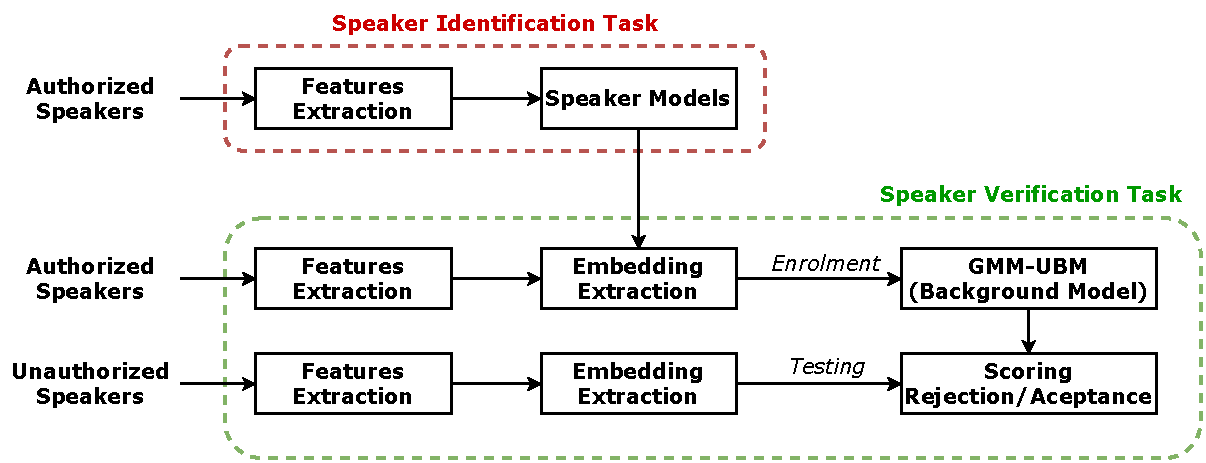
\includegraphics[width=1.0\textwidth]{./architettura.pdf}
    \caption{Architettura del progetto proposta}
    \label{fig:architettura}
\end{figure}
Per quanto riguarda lo score ci basiamo su un valore di soglia sull'EER (Equal Error Rate). La soglia viene utilizzata per decidere quando classificare un'istanza come genuina o impostore. Nel contesto di un sistema di autenticazione biometrica o di rilevamento delle frodi, la soglia è il valore sopra o sotto il quale una decisione viene presa.
Calcolo della soglia (Threshold) alla Equal Error Rate (EER), ovvero il punto in cui il tasso di falsi positivi (FPR) e il tasso di falsi negativi (FNR = 1 - TPR) sono uguali. Si identifica il valore della soglia corrispondente al punto in cui ( FPR - FNR ) è minimo.
Dopo aver calcolato la soglia all'EER, questa viene utilizzata per prendere decisioni di classificazione:
\begin{itemize}
    \item Se il punteggio di un campione è superiore alla soglia, viene considerato normale (positivo)
    \item Se è inferiore alla soglia, viene considerato impostore
\end{itemize}
Un particolare utilizzo di questo sistema potrebbe essere quello di un sistema di riconoscimento biometrico di una azienda, dove solo alcuni dipendenti
sono autorizzati ad accedere (controllo degli accessi), mentre gli altri non devono accedere. E qualora un utente dovesse essere autorizzato ad accedere,
quindi viene verificata la sua identità, il sistema di identificazione associerà un ID che permette di associare a quell'utente i privilegi specifici. \\